\section{引言}

这是论文正文。章节标题使用 \verb|\section{}| 命令，会自动编号。

\subsection{子章节}

子章节用 \verb|\subsection{}| 命令。
引用公式用 \verb|\autoref{eq:example}|，例如 \autoref{eq:example}。

\begin{equation}
    E = mc^2
    \label{eq:example}
\end{equation}

\subsection{图表示例}

如图 \autoref{fig:sample} 所示，插图直接放在 \texttt{img/} 目录下。

\begin{figure}[H]
    \centering
    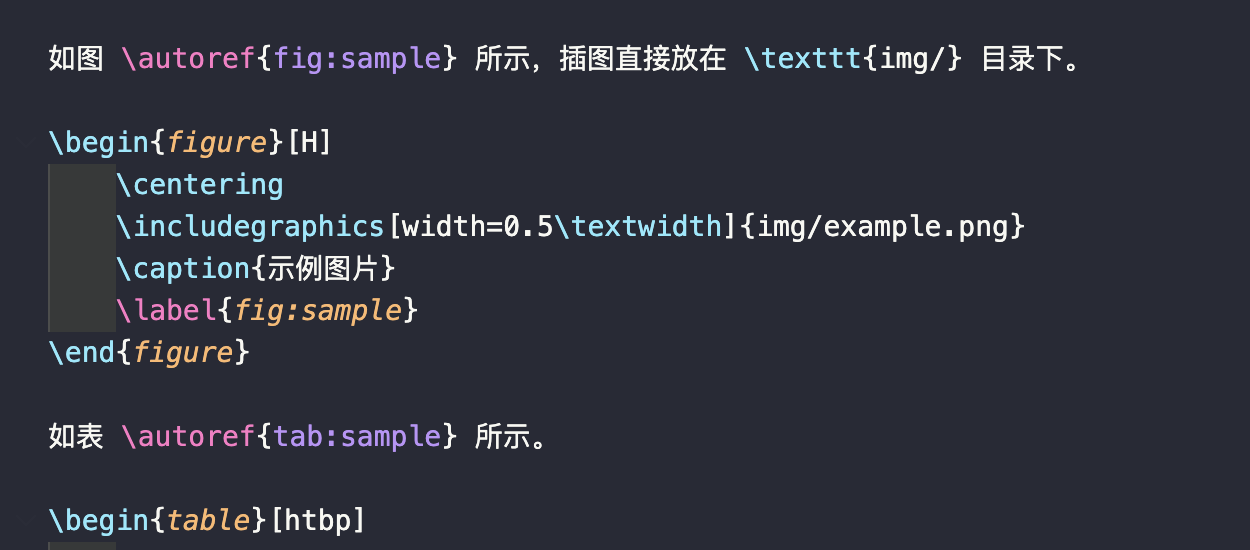
\includegraphics[width=0.5\textwidth]{img/example.png}
    \caption{示例图片}
    \label{fig:sample}
\end{figure}

如表 \autoref{tab:sample} 所示。

\begin{table}[htbp]
    \centering
    \caption{示例表格}
    \begin{tabular}{ccc}
        \hline
        参数 & 符号 & 数值 \\
        \hline
        电阻 & $R$ & $10\Omega$ \\
        电容 & $C$ & $100\mu$F \\
        \hline
    \end{tabular}
    \label{tab:sample}
\end{table}

\subsection{参考文献引用}

使用 \verb|\cite{}| 引用文献，如 \cite{latex-intro} 和 \cite{vscode-latex}。

\section{结论}

本文提供了一个简洁的科技论文写作模板。
